\documentclass[tikz,border=12pt]{standalone}
\usepackage[T1]{fontenc}
\usepackage{mathpazo}
\usepackage{amsmath,amssymb}
\usetikzlibrary{arrows.meta, positioning, calc, fit, decorations.pathreplacing, shapes.geometric, shadows.blur}

\definecolor{stblue}{HTML}{7B97AD}
\definecolor{rwgold}{HTML}{B8995E}
\definecolor{sage}{HTML}{7A9A7E}
\definecolor{dkbrown}{HTML}{3D3530}
\definecolor{wmgray}{HTML}{7B7067}
\definecolor{cream}{HTML}{F9F6F0}
\definecolor{border}{HTML}{D4C9B8}
\definecolor{terracotta}{HTML}{C47A6A}
\definecolor{lavender}{HTML}{907EA0}

\begin{document}
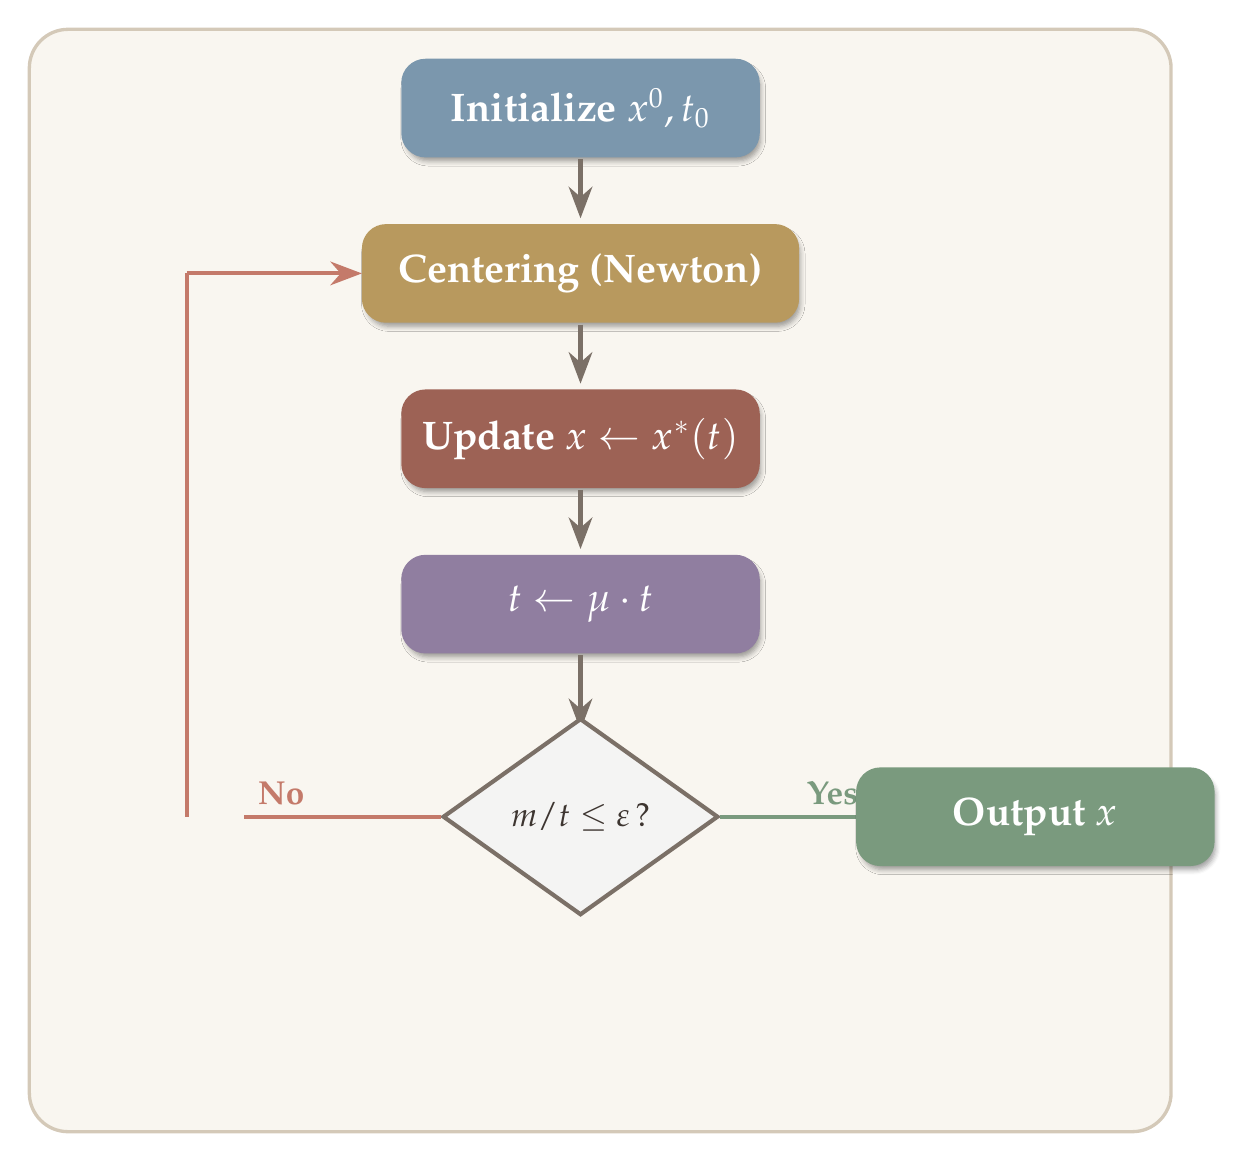
\begin{tikzpicture}[>={Stealth[length=4mm, width=3mm]}, line width=1.5pt,
  box/.style={draw=#1, line width=1.5pt, fill=#1, rounded corners=8pt,
    minimum width=4.5cm, minimum height=1.2cm, text=white, font=\Large\bfseries,
    blur shadow={shadow blur steps=5, shadow xshift=1pt, shadow yshift=-2pt}}]

% Background
\fill[cream, rounded corners=14pt] (-3.0,-0.5) rectangle (11.5,13.5);
\draw[border, line width=1.2pt, rounded corners=14pt] (-3.0,-0.5) rectangle (11.5,13.5);

% Box 1: Initialize
\node[box=stblue] (init) at (4.0,12.5) {Initialize $x^0, t_0$};

% Arrow down
\draw[wmgray, ->, line width=1.5pt] (4.0,11.85) -- (4.0,11.1);

% Box 2: Centering
\node[box=rwgold, minimum width=5.5cm] (center) at (4.0,10.4) {Centering (Newton)};

% Arrow down
\draw[wmgray, ->, line width=1.5pt] (4.0,9.75) -- (4.0,9.0);

% Box 3: Update x
\node[box=terracotta!80!black] (update) at (4.0,8.3) {Update $x \leftarrow x^*(t)$};

% Arrow down
\draw[wmgray, ->, line width=1.5pt] (4.0,7.65) -- (4.0,6.9);

% Box 4: Increase t
\node[box=lavender] (incr) at (4.0,6.2) {$t \leftarrow \mu \cdot t$};

% Arrow down
\draw[wmgray, ->, line width=1.5pt] (4.0,5.55) -- (4.0,4.6);

% Decision diamond
\node[diamond, draw=wmgray, line width=1.5pt, fill=wmgray!8,
      minimum width=3.5cm, minimum height=2.5cm, text=dkbrown, font=\large,
      inner sep=2pt] (decision) at (4.0,3.5) {$m/t \leq \varepsilon$\,?};

% Yes arrow: right
\draw[sage, ->, line width=1.5pt] (decision.east) -- ++(2.8,0);
\node[text=sage, font=\large\bfseries, above] at (7.2,3.5) {Yes};

% Output box
\node[box=sage, anchor=west] (output) at (7.5,3.5) {Output $x$};

% No arrow: left, then up, then right back to Centering
\draw[terracotta, line width=1.5pt] (decision.west) -- ++(-2.5,0);
\node[text=terracotta, font=\large\bfseries, above] at (0.2,3.5) {No};
\draw[terracotta, line width=1.5pt] (-1.0,3.5) -- (-1.0,10.4);
\draw[terracotta, ->, line width=1.5pt] (-1.0,10.4) -- (center.west);

\end{tikzpicture}
\end{document}
